\documentclass{standalone}
\usepackage{tikz}
\begin{document}

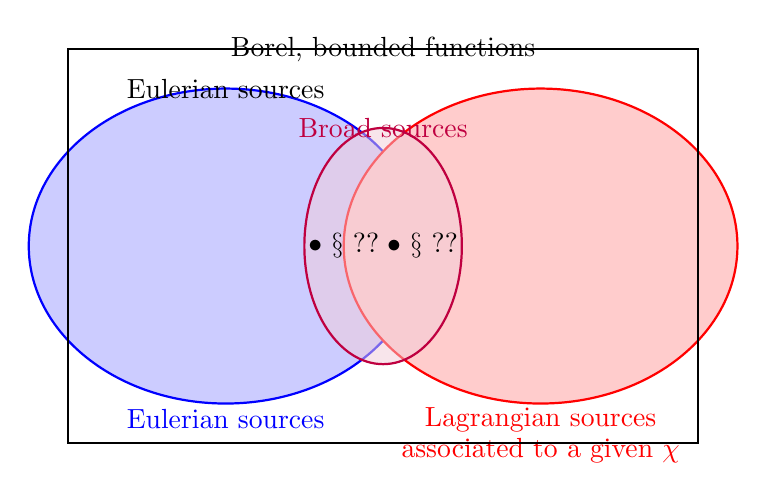
\begin{tikzpicture}
    % Set the background color
    \fill[white] (-4,-2.5) rectangle (4,2.5);
    
    % Draw the Eulerian sources ellipse
    \fill[blue!20] (-2,0) ellipse (2.5 and 2);
    \draw[blue, thick] (-2,0) ellipse (2.5 and 2);
    
    % Draw the Lagrangian sources ellipse
    \fill[red!20] (2,0) ellipse (2.5 and 2);
    \draw[red, thick] (2,0) ellipse (2.5 and 2);
    
    % Draw the intersection area (Broad sources)
    \fill[purple!20, opacity=0.5] (0,0) ellipse (1 and 1.5);
    \draw[purple, thick] (0,0) ellipse (1 and 1.5);
    
    % Add text labels
    \node at (-2, 2) {Eulerian sources};
    \node[blue] at (-2, -2.2) {Eulerian sources};
    \node[red] at (2, -2.2) {Lagrangian sources};
    \node[red] at (2, -2.6) {associated to a given $\chi$};
    \node[purple] at (0, 1.5) {Broad sources};
    
    % Add question marks
    \node at (-0.5, 0) {$\bullet$ $\mathsection$ ??};
    \node at (0.5, 0) {$\bullet$ $\mathsection$ ??};
    
    % Add top label
    \node at (0, 2.5) {Borel, bounded functions};
    
    % Draw the border
    \draw[thick] (-4,-2.5) rectangle (4,2.5);
\end{tikzpicture}

\end{document}